\subsection{Zirkuläre Graphen}
%Wo treten die auf (z.B. Circulant Graphs sind Cayley-Graphen zyklischer Gruppen)
Im Kapitel Warm-up ist uns schon ein zirkulärer Graph begegnet; der Kreis-Graph.\\
Wir nennen einen Graphen zirkulär (engl. "circulant") mit $\,n\,$ Knoten, wenn für $\,n \in \mathbb{N}\,$ und eine Menge $\,I \subset{\{1,..,\lfloor \frac{n}{2} \rfloor \}}\subset{\mathbb{N}}\,$ gilt, dass jeder Knoten $\,v\,$ genau zu jedem Knoten $\,(v+i) (\mod{n})\,$ mit $\,i \in I\,$ benachbart ist; wir bezeichnen solch einen Graphen kurz mit $\,C_n^I$.\;\\
Wir erinnern uns, dass eine $\,(n\times n)$-Matrix zyklisch genannt wird, falls jede Spalte aus der vorherigen durch Anwendung der Permutation $\,(1...n)\,$ hervorgeht.\\
Das ist bei den Adjazenz- und Laplacematrizen von zirkulären Graphen, aufgrund dessen, wann Knoten benachbart sind, der Fall.\\
Zugute kommt uns das bei der Berechnung der Anzahl von Spannbäumen in zirkulären Graphen, denn die Eigenwerte einer zyklischen Matrix sind wohlbekannt.\\
Wir wollen in diesem Zusammenhang folgendes zeigen:
\begin{Tms}
Für die Anzahl der Spannbäume in zusammenhängenden zirkulären Graphen von Grad $\,d\,$ gilt:\\
\begin{equation}
\mathit{k}\left( C_n^I \right) = 
 \begin{cases}
\frac{1}{n} \prod_{j=1}^{n-1} \left(4 \sum_{k \in I} \sin^2 \left( \frac{kj\pi}{n}\right) \right)\qquad\qquad\qquad\qquad\quad\; ,\,falls\,\,\,d\,\,\,gerade\,ist\\
\frac{1}{n} \prod_{j=1}^{n-1} \left(4 \sum_{k \in I/\mathrm{sup}(I)} \sin^2 \left( \frac{kj\pi}{n}\right)-(-1)^j+1\right)\qquad,\,falls\,\,\,d\,\,\,ungerade\,ist
\end{cases}
\end{equation}
\label{tmc}
\end{Tms}
\textbf{Beweis:}\\
Wir beweisen den Satz ähnlich wie \cite{wang_yang_1984}, berechnen daher die Eigenwerte der Laplacematrix und wenden danach Kirchhoffs Matrix-Tree-Theorem an.\\
Für unseren Graphen $\,C_n^I\,$ ist die Laplacematrix zirkulär; wir können sie also durch die erste Spalte eindeutig beschreiben. Der erste Eintrag ist $\,|I|$,\; die Einträge $\,(i+1)\,$  und $\,(n-i)\,$ sind $\,-1\,$ für $\,i \in I$,\; die übrigen $\,0$.\;\\
Des weiteren sind die Eigenwerte von zirkulären Matrizen ein bekanntes Resultat aus der linearen Algebra:
\begin{equation}
 \lambda_j = \sum_{k=1}^{n}l_k\mathrm{exp}{\left(\frac{2\pi \mathrm{i}j(k-1)}{n}\right)}, \,\,\,\,\, {j\in\{0,\ldots,n-1\}}
 \label{cGE}
\end{equation}
$l_k\,$ ist hier der $\,k$-te Eintrag der ersten Spalte.\\ 
Der Eigenwert $\,\lambda_0 = 0$.\; \;  Da der Graph zusammenhängend ist, sind die übrigen Eigenwerte ungleich $\,0\,$ und mit Kirchhoffs Matrix-Tree-Theorem folgt:
\begin{equation}
 \mathit{k}(C_n^I)=\prod_{j=1}^{n-1} \lambda_j
\end{equation}
An dieser Stelle machen wir die Fallunterscheidung, ob der Graph geraden Grad hat, oder nicht.\\
\par
\begingroup
\leftskip=20pt
\rightskip=20pt
\noindent
\textbf{Fall 1:} Grad gerade; das heißt der Grad ist gleich $\,2|I|$\\
Dann ist für alle $\,j \in \{1,\ldots,n-1\}$
\begin{equation}
\begin{aligned}
 \lambda_j = {} & {2|I| - \left( \sum_{k\in I}\left(\mathrm{exp}{\left(\frac{2\pi \mathrm{i}jk}{n}\right)} + \mathrm{exp}{\left(\frac{2\pi \mathrm{i}j(n-k)}{n}\right)}\right)\right)}\\
 = {} & {\left( \sum_{k\in I}\left(\mathrm{exp}{\left(\frac{2\pi \mathrm{i}jk}{n}\right)} - 2 + \mathrm{exp}{\left(\frac{2\pi \mathrm{i}j(n-k)}{n}\right)}\right)\right)}\\
 = {} &-\left( \sum_{k\in I}\left(\mathrm{exp}{\left(\frac{\pi \mathrm{i}jk}{n}\right)} - \mathrm{exp}{\left(\frac{\pi \mathrm{i}j(n-k)}{n}\right)}\right)^2\right)\\
 ={} & 4\sum_{k\in I} \sin^2 \left( \frac{kj\pi}{n}\right)
 \end{aligned}
\end{equation}
,wobei wir die berühmte eulersche Formel verwendet haben.\\
\\ \textbf{Fall 2:} Grad ungerade; das bedeutet der Grad ist $\,2(|I|-1) + 1$\\
Dann gilt für alle $\,j \in \{1,\ldots,n-1\}$
\small
\begin{equation}
\begin{aligned}
 \lambda_j = {} & { 2(|I|-1)+1 - \left(\mathrm{exp}{\left(\frac{2\pi \mathrm{i}j \mathrm{sup}(I)}{n}\right)}+ \sum_{k\in I/\mathrm{sup}(I)}\left(\mathrm{exp}{\left(\frac{2\pi \mathrm{i}jk}{n}\right)}+ \mathrm{exp}{\left(\frac{2\pi \mathrm{i}j(n-k)}{n}\right)}\right)\right)}\\
  = {} &1-\left(\mathrm{exp}{\left(\frac{\pi \mathrm{i}j \mathrm{sup}(I)}{n}\right)} +\sum_{k\in I/\mathrm{sup}(I)}\left(\mathrm{exp}{\left(\frac{\pi \mathrm{i}jk}{n}\right)} - \mathrm{exp}{\left(\frac{\pi \mathrm{i}j(n-k)}{n}\right)}\right)^2\right)\\
  = {} & 4\sum_{k\in I/\mathrm{sup}(I)} \sin^2 \left( \frac{kj\pi}{n}\right)-(-1)^j+1
 \end{aligned}
\end{equation}
\normalsize
Hier sind wir wieder genauso vorgegangen, wie oben.\\
\par
\endgroup
Jetzt kennen wir die Eigenwerte der Laplacematrix und können Kirchhoffs Matrix-Tree-Theorem anwenden; es folgt
\begin{equation}
\mathit{k}\left( C_n^I \right) = 
 \begin{cases}
\frac{1}{n} \prod_{j=1}^{n-1} \left(4 \sum_{k \in I} \sin^2 \left( \frac{kj\pi}{n}\right) \right)\qquad\qquad\qquad\qquad\quad\; ,\,falls\,\,\,d\,\,\,gerade\,ist\\
\frac{1}{n} \prod_{j=1}^{n-1} \left(4 \sum_{k \in I/\mathrm{sup}(I)} \sin^2 \left( \frac{kj\pi}{n}\right)-(-1)^j+1\right)\qquad,\,falls\,\,\,d\,\,\,ungerade\,ist
\end{cases}
\end{equation}
Das wollten wir zeigen.
\begin{flushright} $\,\Box\,$ \end{flushright} 
\begin{Bsps}[$C_n^{1,2}\,$ - Das Quadrat eines Kreises]
\end{Bsps}
Ein berühmtes Beispiel für einen zirkulären Graphen ist $\,C_n^{1,2}$,\, das sogenannte Quadrat eines Kreises (engl. "square of a cycle"). In der Literatur wird dieser Graph auch gelegentlich als $\,C_n^2\,$ bezeichnet. Einen solchen Graphen können wir in Abbildung \ref{c2_8} sehen.
\begin{figure}[H]
  \centering
 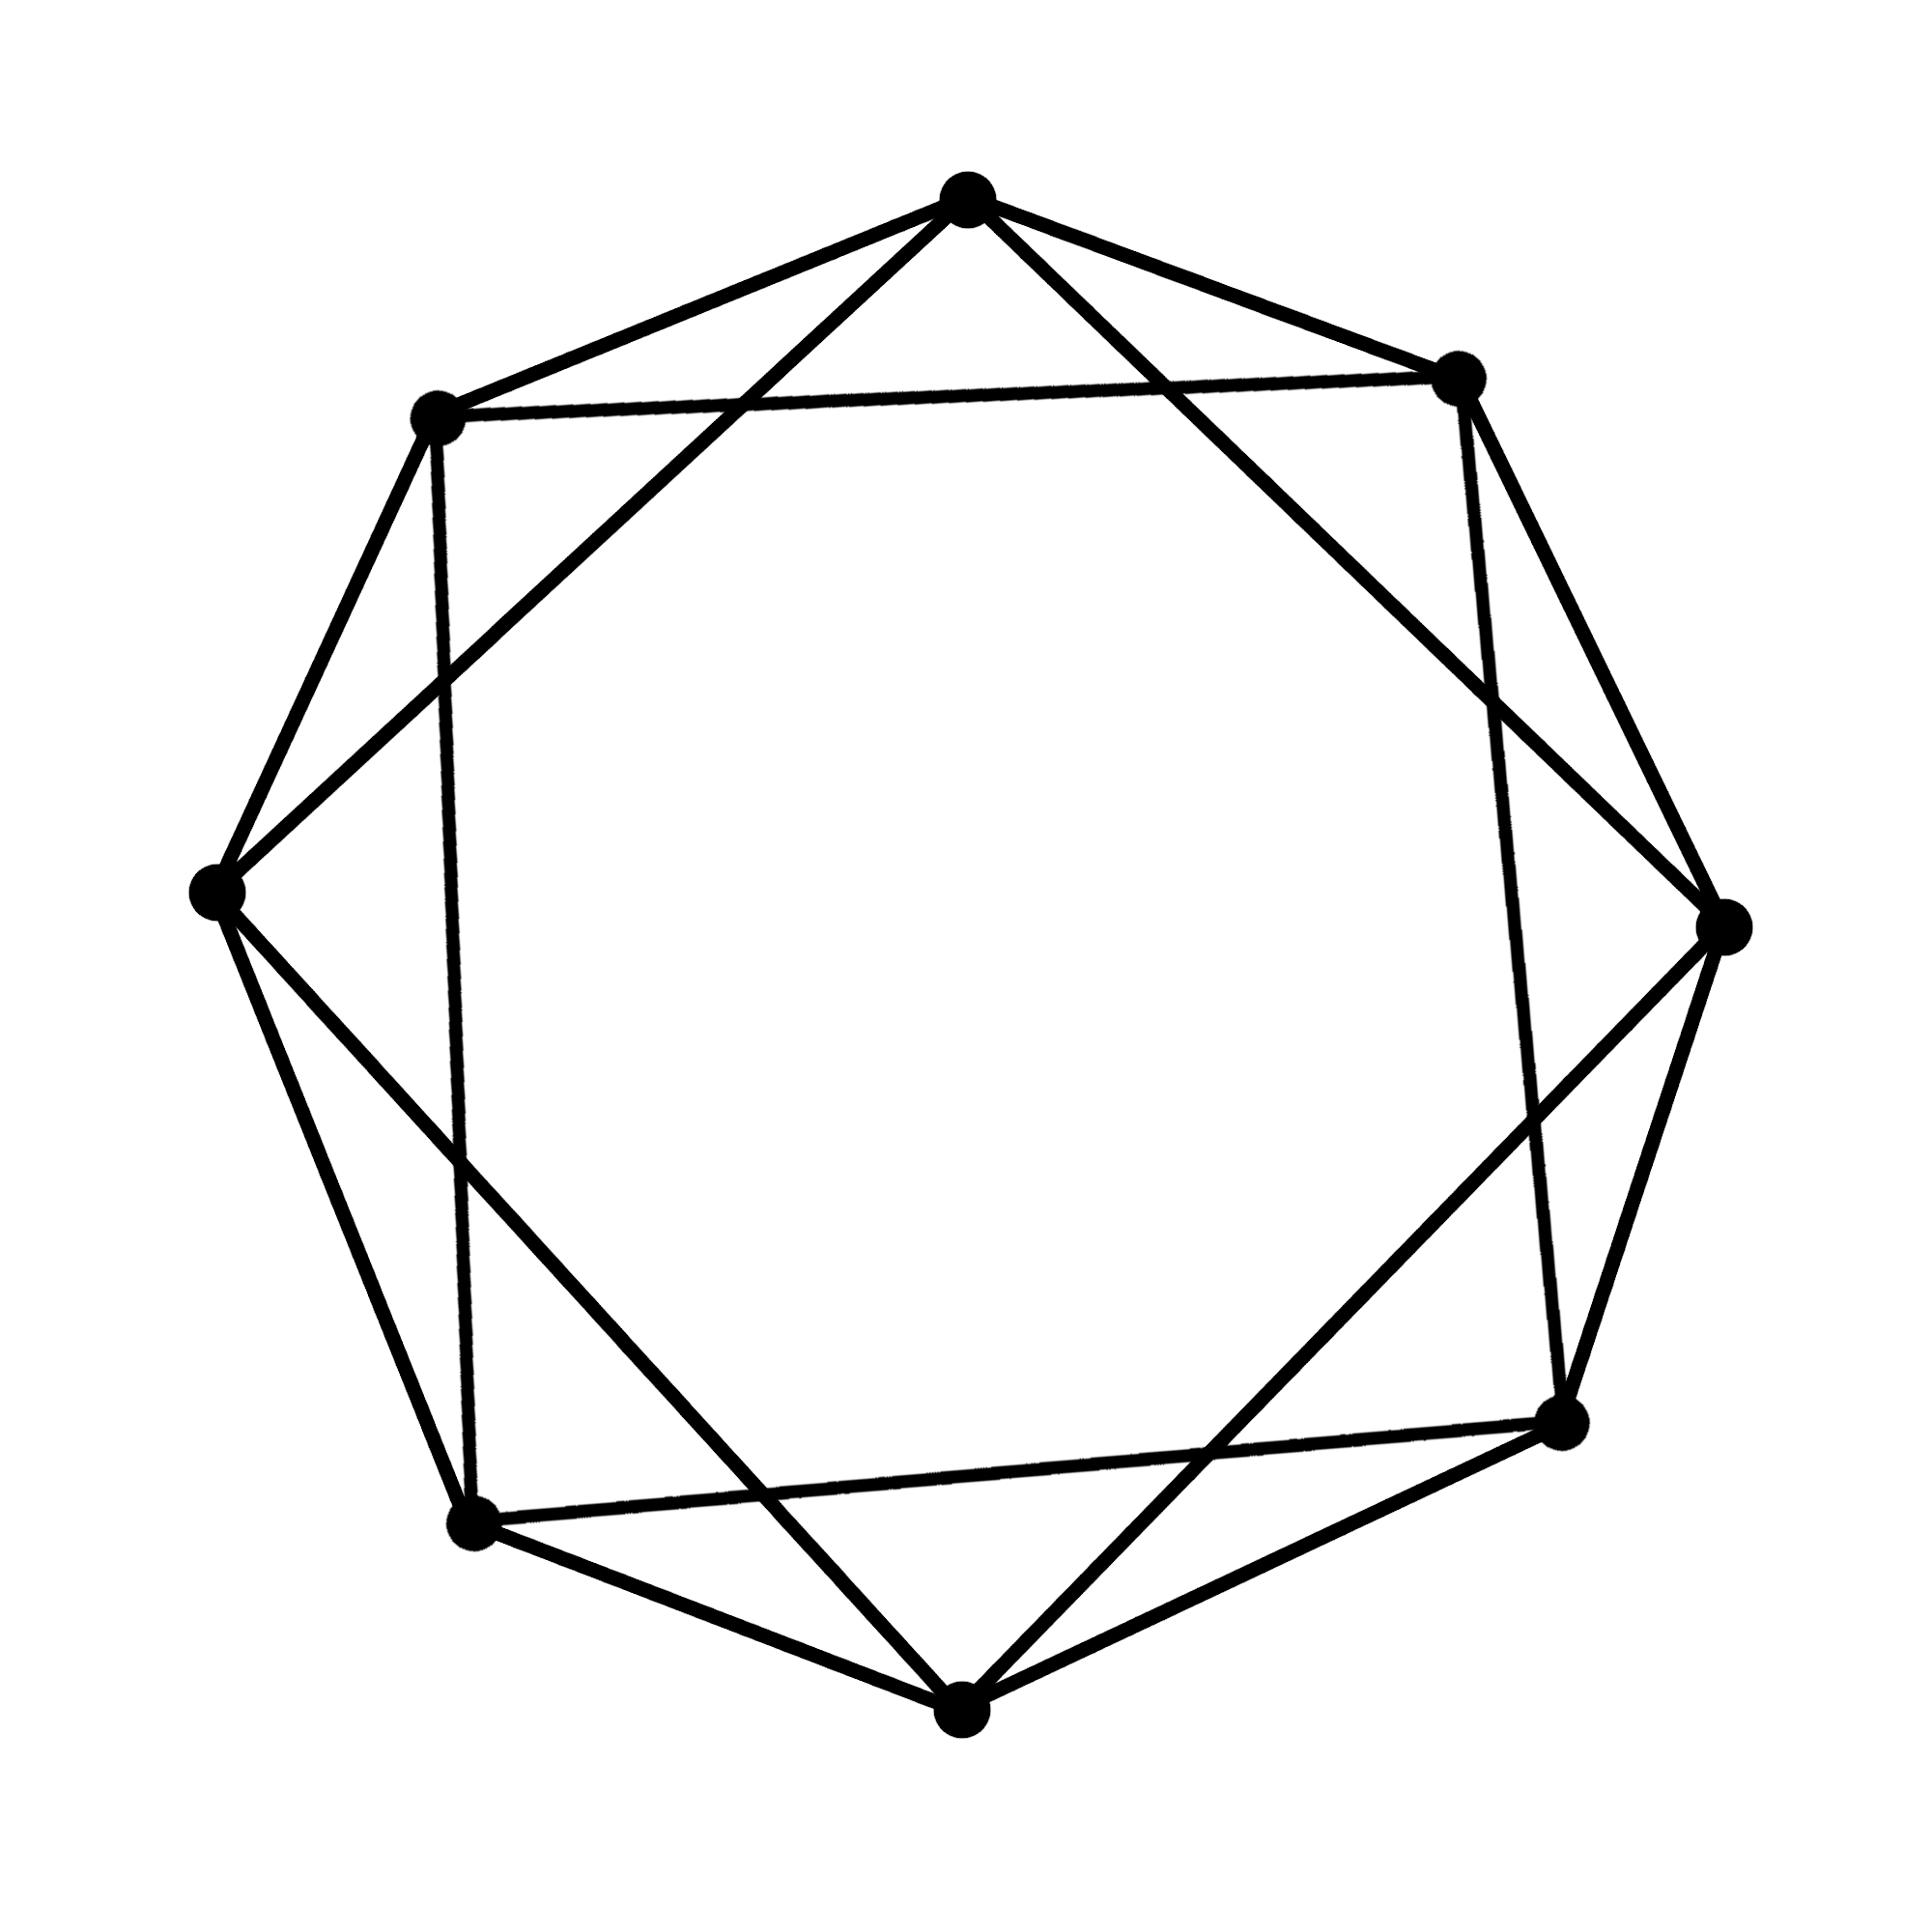
\includegraphics[width=0.5\textwidth]{c2_8.png}
 \caption{$C_8^{1,2}$}
 \label{c2_8} %caption vor label unbedingt
\end{figure}
Bei der Berechnung der Anzahl der Spannbäume des Quadrats eines Kreises stößt man interessanterweise wieder auf die Fibonaccizahlen. Für $\,n\geq5\,$ gilt nämlich
\begin{equation}
 \mathit{k}\left(C_n^{1,2}\right)=n\mathrm{Fib}(n)^2
\end{equation}
Ein Beweis dafür ist nicht schwer, sprengt aber quantitativ den Rahmen für ein Beispiel in dieser Arbeit. Er besteht zum Beispiel daraus sich rekursive Beziehungen von Hilfsmatrizen und Eigenschaften erzeugender Funktionen zunutze zu machen; an dieser Stelle verweisen wir also auf \cite{wang_yang_1984}.

%\todo[inline]{Herleitung Formel}
%Nach der Definition ist $C_n^{1,2}$ (allgemein übliche Bezeichnung $C_n^2$) ein zusammenhängender Graph mit geradem Grad. Wir können also Satz \ref{tmc} anwenden und erhalten
%\begin{equation}
 %\mathit{k}\left( C_n^{1,2} \right) = \frac{1}{n} \prod_{j=1}^{n-1} 4\left(sin^2 \left( %\frac{j\pi}{n}\right) + \sin^2 \left( \frac{2j\pi}{n}\right)\right)
 %= \frac{1}{n} \prod_{j=1}^{n-1} 4\left(sin^2 \left( \frac{j\pi}{n}\right) + 2(\sin^2 \left( %\frac{j\pi}{n}\right)\cos^2 \left( \frac{j\pi}{n}\right)\right))
 %=\frac{1}{n} \prod_{j=1}^{n-1} 4\left(sin^2 \left( \frac{j\pi}{n}\right) 
 %\left(1+\cos^2 \left( \frac{j\pi}{n}\right)\right)\right)
 %= \frac{1}{n} \prod_{j=1}^{n-1} 4\left(sin^2 \left( \frac{j\pi}{n}\right) 
 %\left(2-\sin^2 \left( \frac{j\pi}{n}\right)\right)\right)
 
%\end{equation}

%Im Notfall einen anderen Beweis für $\,C_n^{(1,2)}\,$ raussuchen (eher nicht), der jetzige ist lang, allerdings nutzt er er das MTT was von Vorteil ist (ich werde die Rechnungen verkürzen und nur die wichtigen Teile ausführlich machen, sonst werden das 4-6 Seiten quasi nur mit Rechnungen)
